\chapter{Introduction}
\label{chapter:1}
\section{SimBad project}
The SimBad project (Simulation Birth and Death) is a systems of several programs that simulates cancer cell proliferation. Cancer cell proliferation simply is a  process of cell growth and division. Abnormal cell proliferation, that is, when  cells that divide only finite amount of time before halting their growth or simply dying start untamed proliferation it may cause cancer development.

The SimBad project is a set of programs used to simulate such processes. The simulation process consists of three main steps, each run by separate program. Programs exchange data in pipeline-like way, each component receives some input file (or files) and based on those files it generates some output. The simulation data-flow is depicted on figure \ref{fig:data-flow}. It starts with simulation program \textit{(SimBaD-CLI)} running the simulation and generating stream of output data. In the second step, the stream data is written to file and passed to analyzer program \textit{(SimBaD-analyzer)} for processing. The last step \textit{(SimBad-Reports)} is generating plots and \textit{3D} models from processed data.
The stop condition for simulation process can be certain number of cells in system or elapsed time. For large number of cells, the simulation process can take even several days to finish. For such large simulations to reduce computation time each simulation step can be separated into a dedicated machine - for example in its current state, it can be offloaded to WCSS supercomputer. 
\begin{figure}[h!]
	\centering
		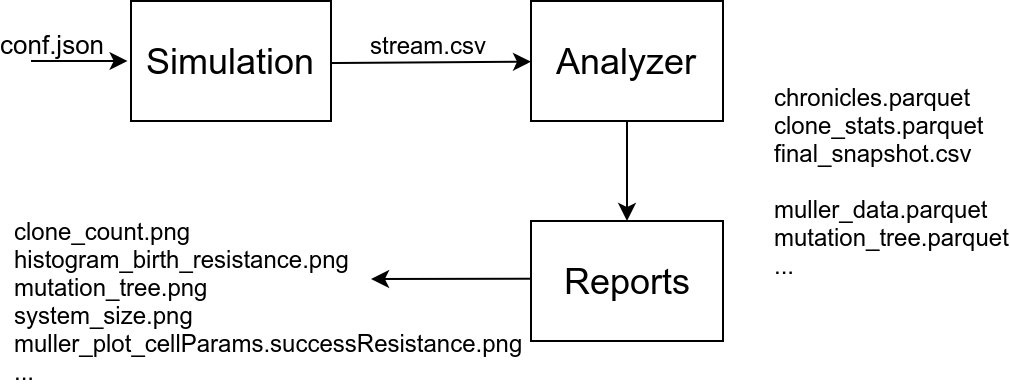
\includegraphics[width=0.9\linewidth]{diagrams/simbad-data-flow.png}
	\caption{Data flow between system components}
	\label{fig:data-flow}
\end{figure}
Although the the unidirectional data flow in system is straightforward, because, the system is very complex, mainly due to installation and configuration. Each step has many dependencies on external libraries that need to be installed on host system and many configuration options that need to be set in order to execute the step. Additionally, the passing of data to each step is not automated, that is the user is responsible for passing valid data to step and triggering its execution. Due to high complexity of system, substantial amount of technical knowledge is needed to run the simulation process, and non-technical user are effectively unable to use this system, without help and guidance of its authors. Moreover, even if the user has required knowledge and skills to install and configure the system, system dependency on third-party code libraries that are not compatible with user machine may prevent the usage of the system. 

To enable to users to use this system, two conditions must be met: the system must be easy to install and easy to control. The purpose of this thesis is to propose and implement an extension to  existing system that will provide a way to install it on user operating system and an easy to use interface that will allow to control and monitor simulation process. This paper will on proposing solution that allows the system to run simulation locally, configured in a way that every system component runs within one host machine, as opposed to more distributed solution. The proposed system was designed with following goals in mind:
\begin{enumerate}
    \item {
        \textit{Ease of use} - the user must be able to install the system and run the simulation on their own (with help from installation instructions and other documentation)
    }
    \item {
        \textit{Non-invasive integration with system} - existing programs will be treated as Black boxes that is viewed only in terms of their inputs and outputs and additional system components will be build on top of existing components without modifying them
    }
    \item {
        \textit{Modular} - each system component should be able to be easily extracted to dedicated environment while preserving the communication link 
    }
    \item {
        \textit{OS agnostic installation} - the system must be possible to install on most popular operating systems (Linux, Windows, Mac OS)
    } 
    \item{
        \textit{Configured out-of-the-box but configurable} - zero-configuration needed for normal user and extensive configuration available to power user
    }
\end{enumerate}
\section{Thesis structure}
The structure of this thesis is as follows. Chapter 2 will be analyze existing components and its dependencies and discuss the ways of making the system host-agnostic. Chapter 3 will give an high level overview of proposed architecture, its design decisions with regards to goals and chosen technologies with substantiations. In chapter 4 each additional component that was proposed in chapter 3 will be discussed in more detail. 